% Full title as you would like it to appear on the page
\chapter{Expression variation and covariation impair analog and enable binary signaling control}
% Short title that appears in the header of pages within the chapter
\chaptermark{Analog vs Binary Signaling Control}

\section{Abstract}
Due to noise in the synthesis and degradation of proteins, the concentrations of individual vertebrate signaling proteins were estimated to vary with a coefficient of variation (CV) of approxi- mately 25\% between cells. Such high variation is beneficial for population-level regulation of cell functions but abolishes accurate single-cell signal transmission. Here, we measure cell-to-cell vari- ability of relative protein abundance using quantitative proteomics of individual Xenopus laevis eggs and cultured human cells and show that variation is typically much lower, in the range of 5–15\%, compatible with accurate single-cell transmission. Focusing on bimodal ERK signaling, we show that variation and covariation in MEK and ERK expression improves controllability of the percentage of activated cells, demonstrating how variation and covariation in expression enables population-level control of binary cell-fate decisions. Together, our study argues for a control principle whereby low expression variation enables accurate control of analog single-cell signaling, while increased variation, covariation, and numbers of pathway components are required to widen the stimulus range over which external inputs regulate binary cell acti- vation to enable precise control of the fraction of activated cells in a population.
Keywords

\section{Introduction}
Vertebrate signaling has been shown to control both binary and analog outputs. Here, we use the term binary if the output is bimodal and the term analog if the output signal changes in parallel with the input signal without bifurcations during the transmission. Examples of binary signaling decisions include the commitment to start the cell cycle (Cappell et al, 2016), cell differentiation (Chang et al, 2008; Jukam & Desplan, 2010; Ahrends et al, 2014), apoptosis
(Spencer et al, 2009), action potentials (Hodgkin & Huxley, 1952) and the explosive secretory response of mast cells when encounter- ing an antigen (Hide et al, 1993). Effective analog signaling in individual cells has been observed, for example, in the visual trans- duction system where the number of absorbed photons proportion- ally increases electric outputs in cone cells (Arshavsky et al, 2002), in single-cell IP3 and Ca2+ regulation by GPCRs (Nash et al, 2001), as well as for CD-8 (Tkach et al, 2014) and IL-2 signaling (Feinerman et al, 2008) in T cells. Analog signaling is also needed to accurately regulate the timing or duration of intermediate cell processes such as in the cell cycle where the time between the start of S-phase to mitosis has only small variation between individual cells (Spencer et al, 2013). Such precise regulation of durations requires low noise in the signaling steps before mitosis (Kar et al, 2009). Together, these examples suggest that accurate analog signal- ing is important for graded control of cell outputs in single cells as well as for accurate internal timing. A main motivation for our study was the high levels of protein expression variation that have been reported in vertebrate cells with coefficient of variations (CVs) of approximately 25\% (Sigal et al, 2006; Spencer et al, 2009; Gaudet et al, 2012). Such high levels of expression variation are beneficial for binary signaling which is often regulated at the population level rather than single-cell level. In population-based signaling, a goal of organisms is to use different levels of input to regulate the percentage of cells in a population that make a binary decision such as whether to proliferate, differentiate, or secrete. For input stimuli to control which percentage of cells are activated, high noise in signaling is needed between cells in the population such that individual cells have different sensitivities to input stimuli (Su¨el et al, 2007; Raj & van Oudenaarden, 2008; Kalmar et al, 2009; Eldar & Elowitz, 2010; Ahrends et al, 2014). However, the same high noise needed to control population-level signaling does not have any benefit for analog signaling and just serves to degrade signal transmission. These different demands on noise for analog and binary signaling suggest that there is a trade- off for noise between population-level and single-cell signaling (Suderman et al, 2017). Specifically, the reported high levels of expression variation and signaling noise in mammalian cells (Sigal et al, 2006; Cheong et al, 2011; Gaudet et al, 2012; Selimkhanov et al, 2014) raise the question of how noise in a signaling system can be low enough for accurate analog signaling. It also remained unclear how the different potential internal noise sources couldgenerate optimal conditions for analog single-cell versus binary population-level signaling. Here, we measure cell-to-cell variation in the relative abundance
of pathway components to understand the limits of analog and binary signaling accuracy. We also investigated the role of covaria- tion of pathway components since we realized that covariation could exacerbate the analog signaling problem and/or enable the control of population-level binary signaling. We considered that previous estimates of cell-to-cell variation in protein expression might be too high due to experimental challenges in accurately measuring small differences in protein abundance between cells and accounting for “hidden variables” such as differences in cell size and cell cycle state (Symmons & Raj, 2016). To determine lower limits of protein variation, we developed single-cell quantitative proteomics methods in single Xenopus laevis eggs and employed quantitative normalization of cultured human cells to accurately measure variations in protein abundance normalized by protein mass. We found that cell-to-cell variation in relative protein abundance is much lower than expected, with CVs of between 5 and 15\%, suggesting that expression variation is less limiting than currently believed and is compatible with accurate analog signal transmission. Furthermore, our simulations show that these exper- imentally observed low levels of expression variation pose a chal- lenge for cells to accurately control population-level decisions. One potential strategy to increase pathway output variation was revealed by experiments which showed significant covariation between the single-cell expression of two sequential signaling components, MEK and ERK. Our modeling showed that such increased covariation—which increases the overall noise in the signaling pathway—allows populations of cells to control the percentage of cells that activate ERK over a wider range of input stimuli, suggesting that covariation of signaling components is one strategy for populations of cells to more accurately control binary cell-fate decisions. Finally, we developed a metric to describe how systems can optimize the shared use of pathway components to control single-cell analog and population-level binary signal trans- mission by using different numbers of regulatory components, levels of expression variation, and degrees of covariation.

\section{Results}
\subsection{Computational simulations using reported levels of expression variation show a dramatic loss of analog single-cell transmission accuracy}
Here is a reference to Figure \ref{fig:paper1_fig1}.
We found bacteria, roughly 5 \si{\mu}m in length, that live at 95\degree C for roughly 90\% of the year. More symbols: \$, \#, 10\textsuperscript{5}, $\alpha$, $\beta$, $\gamma$, $\kappa$, \textbf{bold}, \textit{italics}.
Quotation marks are "correctly oriented" thanks to the csquotes package.
Now an inline equation: $E = mc^2$. Now a reference to Equation \ref{eqn:paper1_eqn1}:
\begin{equation}\label{eqn:paper1_eqn1}
d_t = \frac{c - pn_t}{n_t}
\end{equation}

\begin{figure}[hbt!]
\centering
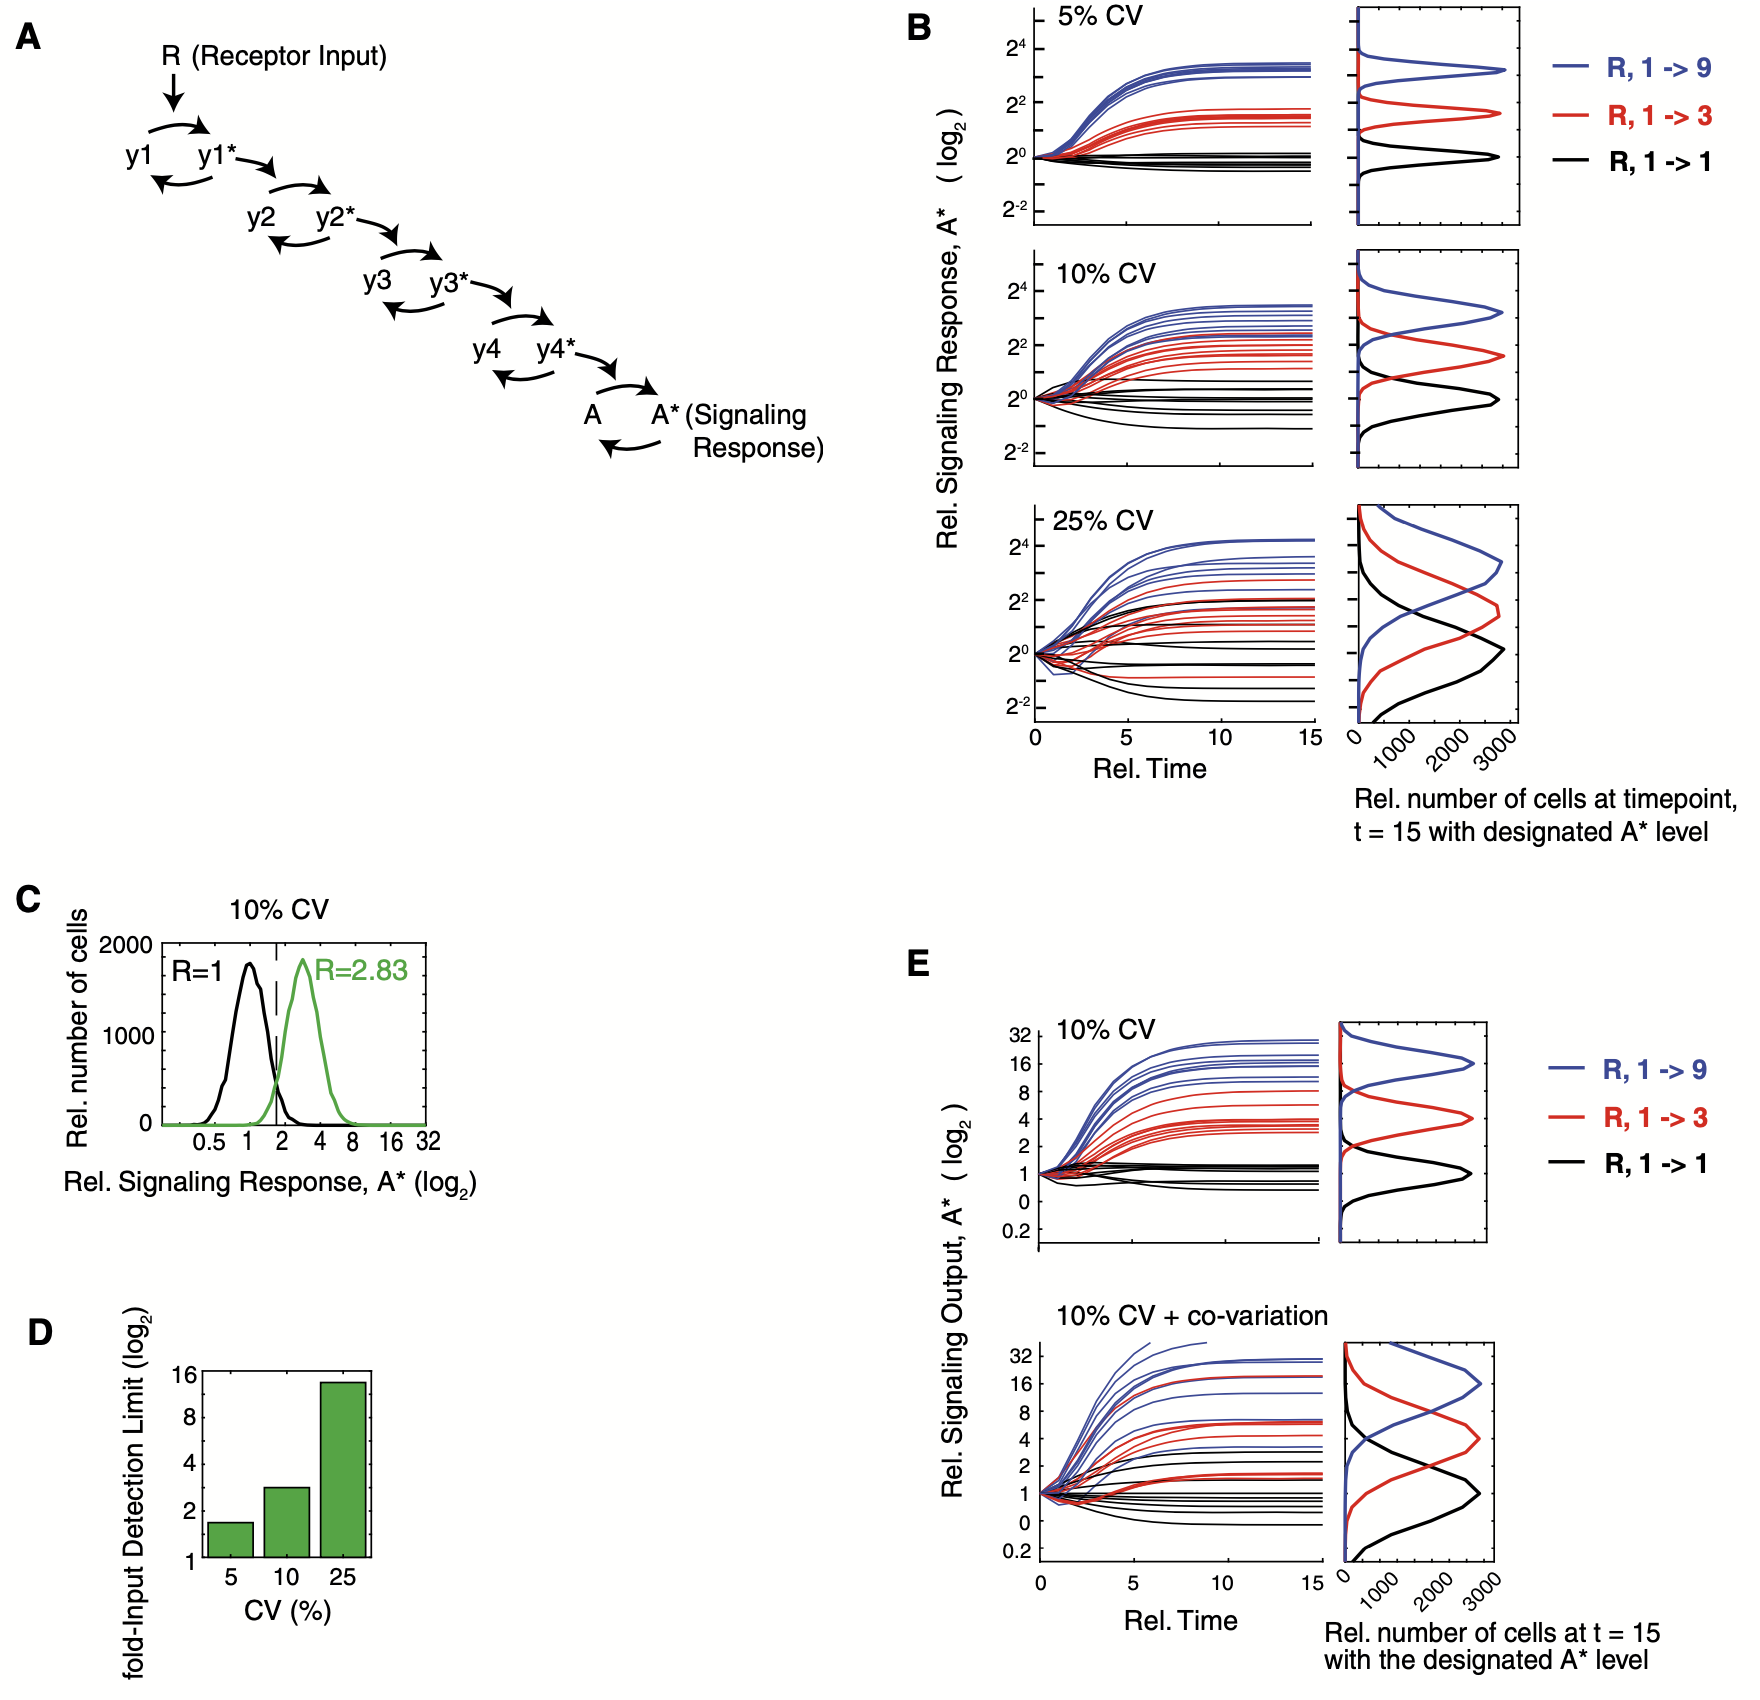
\includegraphics[width=14cm, keepaspectratio]{figs/paper1/fig1.png}
\caption[Short figure caption for List of Figures]{Long figure caption text that explains everything.}
\label{fig:paper1_fig1}
\end{figure}

There will be more text here.

More text here.

More text here.

More text here.

More text here.

More text here.

\subsection{Result 2}
We discovered something else. Here is a reference to Table \ref{tab:paper1_tab1}.

\renewcommand{\arraystretch}{2}  % make spacing nicer
\begin{table}[hbt!]
\centering
\begin{tabularx}{\textwidth}{c|c|c|c}  % 4 columns center-justified
   \textbf{Col 1} & \textbf{Col 2} & \textbf{Col 3} & \textbf{Col 4} \\
   \hline  % horizontal line
   Text in Row 1a & Text in Row 1b & Text in Row 1c & Lots of text in Row 1d \\
                  & Row 1.5b & Row 1.5c & Row 1.5d \\
   \hline
   Row 2a & Row 2b & Row 2c & Row 2d \\
   \hline
   Row 3a & Row 3b & Row 3c & Row 3d \\
\end{tabularx}
\caption[Short table caption for List of Tables]{Long table caption explaining everything.}
\label{tab:paper1_tab1}
\end{table}

More text here.

More text here.

More text here.

More text here.

\begin{sloppypar}
FixAwkwardSpacingWithSloppypar FixAwkwardSpacingWithSloppypar FixAwkwardSpacingWithSloppypar FixAwkwardSpacingWithSloppypar FixAwkwardSpacingWithSloppypar.
\end{sloppypar}

More text here.

More text here.

\section{Conclusions}
The end of the paper.
